\section{Problem 3}
\subsection{(a)}

\begin{minted}[linenos, bgcolor = bg]{python}

    for i in range(nexp):
    # simulates n realizations from a Gaussian 
    # with mean mu and var sigma^2
    x = np.random.normal(mu,sigma,n)
    # TODO: adapt for b)
    sig = np.sqrt(np.var(x, ddof=1))
    # computes the 0.5% quantile of a Gaussian, roughly -2.576  
    fac1 = scipy.stats.norm.ppf((1-gamma)/2, 0, 1) 
    # computes the 99.5% quantile of a Gaussian, roughly 2.576
    fac2 = scipy.stats.norm.ppf((1-gamma)/2 + gamma, 0, 1) 

    # computes the 0.5 quantile using the t-test
    fac3 = scipy.stats.t.ppf((1+gamma)/2, n-1)
    # computes the 99.5 quantile using the t-test
    fac4 = scipy.stats.t.ppf((1+gamma)/2-gamma, n-1)
    xmean = np.mean(x) # Sample mean
    a = xmean - fac2*sig/np.sqrt(n) 
    b = xmean - fac1*sig/np.sqrt(n) 
    ac = xmean - fac3*sig/np.sqrt(n) # TODO: adapt for c)
    bc = xmean - fac4*sig/np.sqrt(n) # TODO: adapt for c)
\end{minted}

\begin{figure}[H]
    \centering
    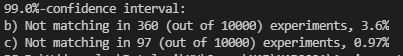
\includegraphics[width=0.9\textwidth]{Figures/result_of_confidence.JPG}
    \caption{Result from 10000 experiments}
\end{figure}